%課題研究レジュメテンプレート ver. 1.2

\documentclass[uplatex]{jsarticle}
\usepackage[top=20mm,bottom=20mm,left=20mm,right=20mm]{geometry}
\usepackage[T1]{fontenc}
\usepackage{txfonts}
\usepackage{wrapfig}
\usepackage[expert,deluxe]{otf}
\usepackage[dvipdfmx,hiresbb]{graphicx}
\usepackage[dvipdfmx]{hyperref}
\usepackage{pxjahyper}
\usepackage{secdot}

\makeatletter
  \renewcommand{\section}{%
    \if@slide\clearpage\fi
    \@startsection{section}{1}{\z@}%
    {\Cvs \@plus.5\Cdp \@minus.2\Cdp}% 前アキ
    {.5\Cvs \@plus.3\Cdp}% 後アキ
    %{\normalfont\Large\headfont\raggedright}}
    {\normalfont\raggedright}}

  \renewcommand{\subsection}{\@startsection{subsection}{2}{\z@}%
    {\Cvs \@plus.5\Cdp \@minus.2\Cdp}% 前アキ
    {.5\Cvs \@plus.3\Cdp}% 後アキ
    %{\normalfont\large\headfont}}
    {\normalfont}}

  \renewcommand{\subsubsection}{\@startsection{subsubsection}{3}{\z@}%
    {\Cvs \@plus.5\Cdp \@minus.2\Cdp}%
    {\z@}%
    %{\normalfont\normalsize\headfont}}
    {\normalfont}}
\makeatother
%ここから上を編集する必要はない.






\title{\vspace{-14mm}}
\author{PMコース 矢吹研究室 1442043 川崎 貴雅}
\date{}%日付を入れる必要はない.
\pagestyle{empty}%ページ番号は振らない.
\begin{document}
\maketitle





\section{研究の背景}

グロバール化と騒がれる今の世の中では,地方創生を急がなくてはならない状況である.

日本の中小企業は,質の高い製造技術を有しているが,知的財産や商品アイディアなどを持たない企業が多数存在している.それとは逆に大企業や大学,研究機関はニーズに基づいた発想にもかかわらず,市場規模の小ささなどから使われない特許が多数存在している.

このような未使用の特許の中には開放特許というものがある.開放特許は商品開発からスタートできるメリットなどがあるが,開放特許は十分に活用されていないというのが現状である.

これは開放特許を活かすことのできる仕組みというのが出来上がっていないことが原因であると考えられる.
これの解消するためにはは地域にある中小企業と地域産業支援機関や大学に金融機関などが互いに持つ資源を活用することが重要である.\cite{self}

この例としてはさいたまモデル事業というものがあり,中小企業の自社製品開発力を引き上げることと技術移転を後押しすることが狙いである.

つまるところさいたまモデルとは,開放特許と中小企業を結びつけ,試作品開発から商品化,販売段階まで支援することなのである.

また事業の目標を地域の活性化と商品の販売による利益の創出としているため,地域の支援機関とと切れ目のない支援体制を構築して成果を出すのである.

さいたまモデル事業の例としてはやしお毎日一万歩運動や貯筋してこころもからだも元気・健康!などがある.\cite{self2}



\section{研究の目的}

本研究の目的は,富士通の解放特許技術を活用して,オリンピックやパラリンピックに地方創生,災害の被災地支援を意識した斬新な商品アイディアを提示し,中小企業の新事業の足掛かりになる事である.

\section{プロジェクトマネジメントとの関連}

本研究のプロジェクトはプロジェクトマネジメントの10個の知識エリアのうち,人的資源マネジメントとコストマネジメントに特に関連する.

人的支援マネジメントは他学科の学生とかかわることからしっかりとしたチームビルディングが要求されるため,コストマネジメントが中小企業に提案したときに資金的な問題がかかわるため主に関連づけられる.


\section{研究の方法}

ビジネス発表会の日程と内容.

\begin{itemize}
\item 8月2日・・・キックオフ.ビジネスアイディア発表会に参加する学生が顔合わせとビジネスアイディア発表会の内容や使用する富士通の特許を確認する.
\item 9月8,12,15日・・・ワークショップ.富士通の視線検知技術を使いアイディアだしやニーズを調べる.
\item 9月17日・・・グループ作成.指定されたメンバーで顔合わせする.
\item 10月5日・・・アイディアシート提出.作成されたグループ内で出したアイデアの概要を指定されたシートに記入して提出する.
\item 10月11日・・・中間発表.資料を作成し提出する,アイディアを選んだ理由や特許をどのように活用してるのかを中心に進捗を報告する.
\item 11月11日・・・最終発表.資料を作成し中間発表の内容に収益構造やサービスデザインなどを紹介する.
\end{itemize}

作業分担

グループ作成からアイディアシート提出の間の分担は,デザイン科学科のメンバーがアイデアだしとイメージをイラストなどにしてもらいアイディアシートに記載する.
プロジェクトマネジメント学科のメンバーはアイディアだしと大まかな事業内容を考えアイディアシート記載する.

デザイン科学科が中間発表,最終発表資料を制作する.
プロジェクトマネジメント学科が金銭設定,プレゼンテーションをする.

\section{現在の進捗状況}

%\begin{wrapfigure}[行数]{r}{幅}%行数はオプションだが,調整しないとうまくいかない.
\begin{wrapfigure}[11]{r}{8cm}
\vspace*{-\intextsep}
%\includegraphics[width=図の幅,clip]{ファイル名}\label{参照用ラベル}
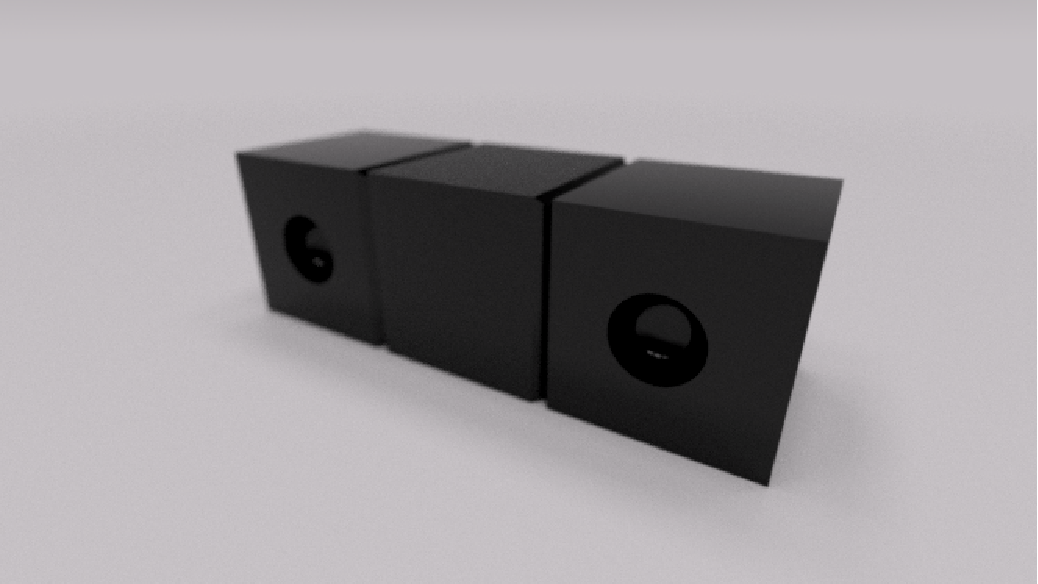
\includegraphics[width=8cm,clip]{design.pdf}
\caption{プロジェクト内で考えたハードのデザイン}\label{サンプル図}
\end{wrapfigure}

8月2日から始まったビジネスアイディアは11月11日の最終発表が終了して,プロジェクトが完了してる.
ビジネスアイディア発表会で制作,提出した成果物は以下の通りとなっている.

%\begin{wrapfigure}[行数]{r}{幅}%行数はオプションだが,調整しないとうまくいかない.
\begin{wrapfigure}[11]{r}{8cm}
\vspace*{-\intextsep}
%\includegraphics[width=図の幅,clip]{ファイル名}\label{参照用ラベル}

\includegraphics[width=8cm,clip]{f.pdf}
\caption{プロジェクト内で考えたアプリケーションのロゴ}\label{サンプル図}
\end{wrapfigure}

\begin{itemize}
\item アイディアシート
\item ハードウェア,アプリケーションのロゴデザイン
\item ハードウェアのデザインサンプル品
\item 中間,最終発表用資料
\end{itemize}

\section{今後の計画}

プロジェクト自体が終了しているため計画はないが今回のプロジェクトで反省点をあげる.

\begin{itemize}
\item 提出物の完成が遅くなり提出がぎりぎりになってしまった.
\item 学科が違うことでslackでのやり取りが多かったが意思疎通に齟齬などによる相違点の確認が甘く資料にミスが出た.
\item テーマ内容の詳細確認をしなかったため意見のすれ違いが起きて進捗に遅れが出た.
\end{itemize}

上記3つから背景で記載した通り,違う学科の学生とプロジェクトを行うことで考え方の違いなどの差を感じれたため良い経験になったとともに,事前に回避できた問題もあったためこのような機会が今後あるか定かではあるが,次からは早急に対処できるように対策を考えている.



\bibliographystyle{junsrt}
\bibliography{biblio}%「biblio.bib」というファイルが必要.

\end{document}

